\documentclass[a4paper]{article}
\usepackage{amsmath}
\usepackage{amssymb}
\usepackage{xcolor}
\usepackage{amsthm}
\usepackage{dsfont}
\usepackage{graphicx}
\usepackage{subcaption}
\usepackage{hyperref}
\usepackage{datetime}
\usepackage{outlines}
\usepackage[round]{natbib}   % omit 'round' option if you prefer square brackets

\usepackage{matlab-prettifier}

\newdateformat{monthyeardate}{\monthname[\THEMONTH] \THEYEAR}

\newcommand{\newmarkedtheorem}[1]{%
  \newenvironment{#1}
    {\pushQED{\qed}\csname inner@#1\endcsname}
    {\popQED\csname endinner@#1\endcsname}%
  \newtheorem{inner@#1}%
}

\theoremstyle{definition}
%\newtheorem{eg}{Example}[section]
\newmarkedtheorem{eg}{Example}[section]
\newtheorem{observation}{Observation}[section]
\newtheorem{define}{Definition}[section]
\theoremstyle{plain}
\newtheorem{proposition}{Proposition}[section]
\newtheorem{theorem}{Theorem}[section]
\newtheorem{assump}{Assumption}
\newtheorem{remark}{Remark}

\author{Jeroen van Riel}
\date{\monthyeardate\today}
\title{Explicit Trajectory Generation}

\begin{document}

\begin{figure}
  \centering
  \makebox[\textwidth][c]{% wider than textwidth
    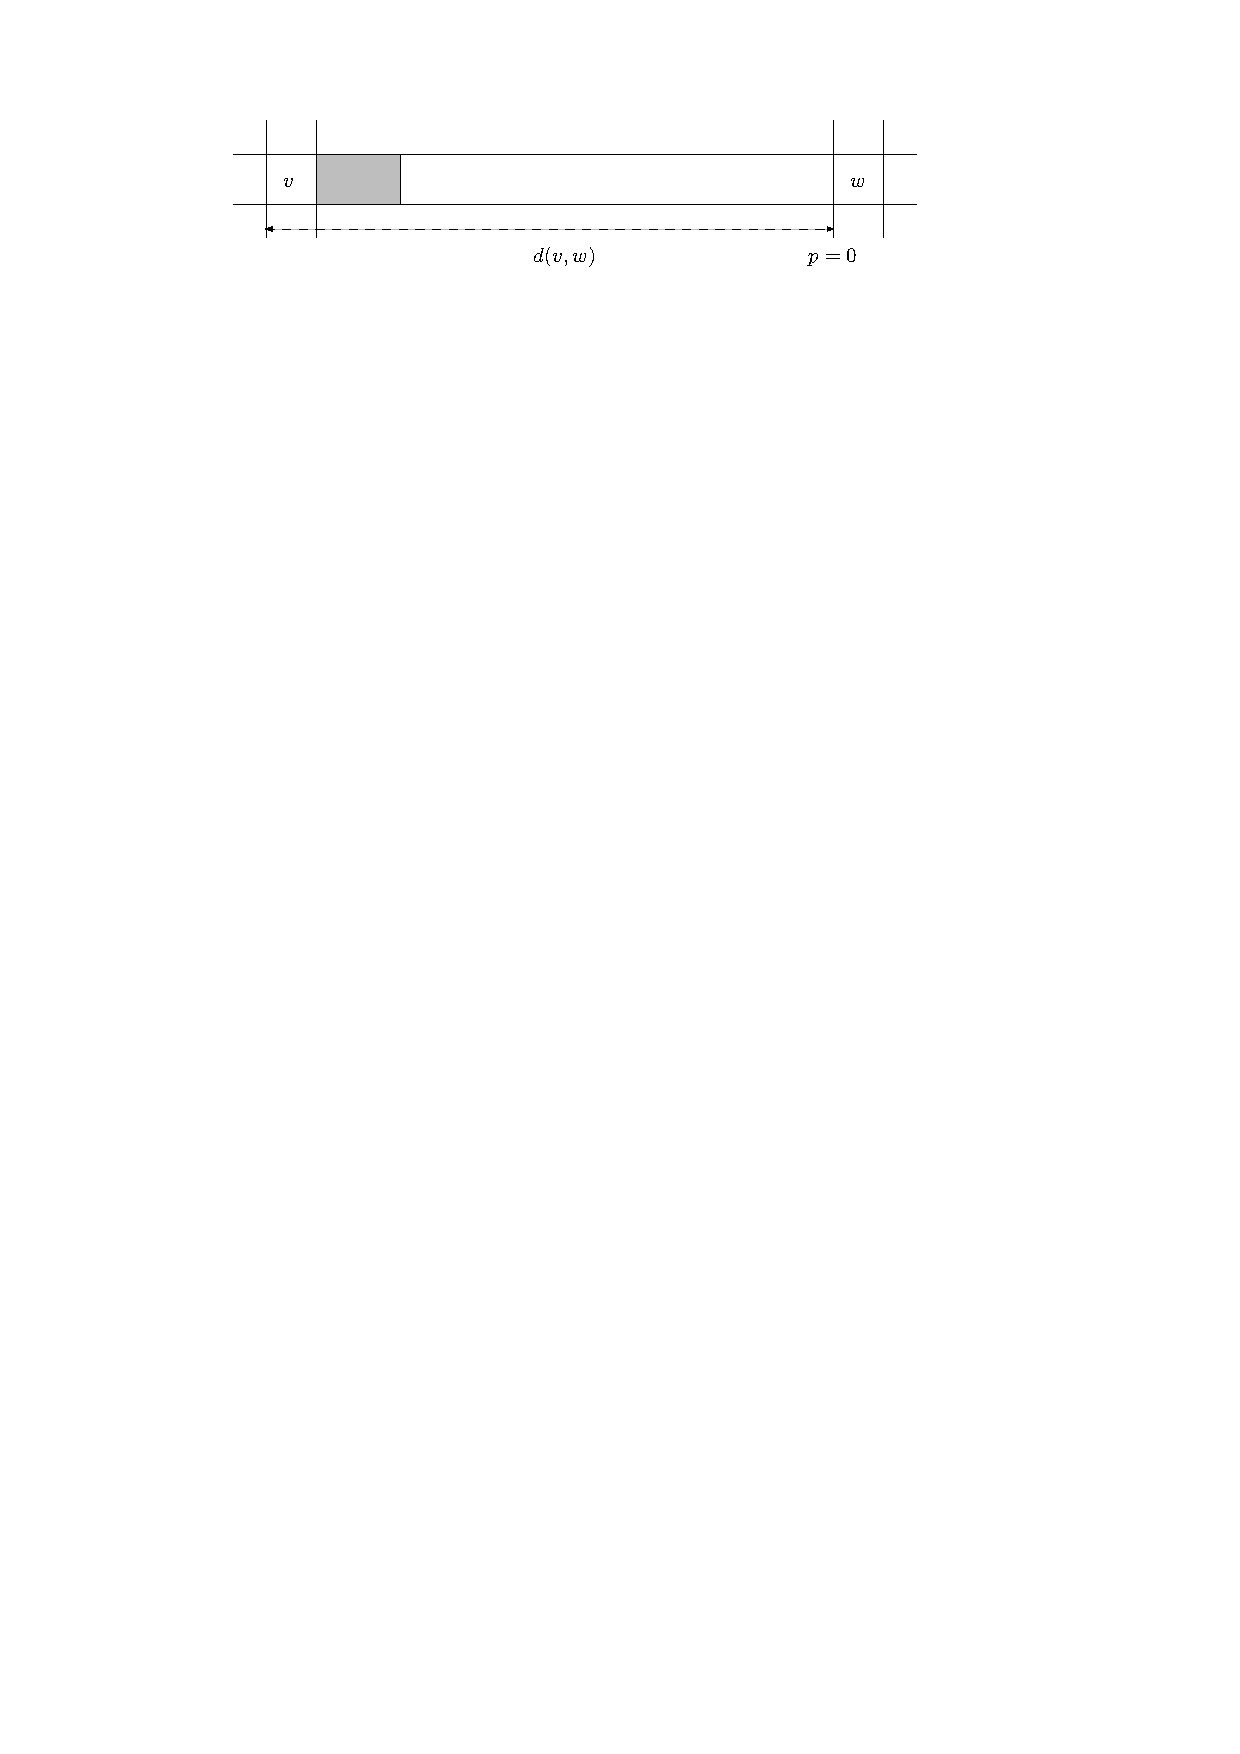
\includegraphics[width=1.1\textwidth]{figures/motion/tandem}
  }
  \caption{Tandem of two intersections $v$ and $w$ with lane of length $d(v,w)$.
    The grey rectangle represents some vehicle that just left intersection $v$.}
  \label{fig:tandem}
\end{figure}

\section*{Trajectory of single vehicle}

% motivation for model
We need to take into account the fact that a lane between two consecutive
intersections has finite capacity for vehicles, in order to model possible
blocking effects, also known as \textit{spillback}.

% define tandem model
We start with the simplest extension of the single intersection model by
considering two intersections in tandem, as illustrated in
Figure~\ref{fig:tandem}. Let $v$ denote the left intersection and $w$ the right
intersection and assume that vehicles drive from left to right. Let the length
and width of a vehicle $i$ be denoted by $L_{i}$ and $W_{i}$, respectively. We
measure the position of a vehicle at the front bumper and we let position $x=0$
be at the stopline of intersection $v$. We denote the position of the stopline
at $w$ by $x=x_{f}=d(v,w)$. To simplify the following discussion, we assume that all
vehicles have the same dimensions.

\begin{assump}
  \label{assump1}
  All vehicles have the same length $L_{i} = L$ and width $W_{i} = W$.
\end{assump}

Now assume that some vehicle is scheduled to cross $v$ at time $t=0$ and to
cross $w$ at some time $t_{f}$. Let $y(t)$ denote the trajectory of the
predecessor, assuming there is one. In order to keep the vehicle as close to $w$
as possible at every time, we can generate a trajectory by solving the optimal
control problem
\begin{equation}
  \begin{aligned}
  \max_{x}    \quad & \int_{t=0}^{t_{f}} x(t) dt \\
  \begin{alignedat}{2}\text{s.t.}\\ {}\end{alignedat} \quad &\begin{alignedat}{2}
                     0 \leq \; &\dot{x}(t) \leq v_{\max} , \\
                     {-a_{\max}} \leq \; &\ddot{x}(t) \leq a_{\max} , \\
                    y(t) \leq \; & x(t) , \label{eq:follow} \\
                    \end{alignedat} \\
                    &\begin{alignedat}[t]{2}
                    & x(0) = 0 , &&  x(t_{f}) = d(v,w) , \\
                    & \dot{x}(0) = v_{\max} , \;\; && \dot{x}(t_{f}) = v_{\max} .
                    \end{alignedat}
  \end{aligned}
\end{equation}
%
We believe that the optimal control is always ``bang-bang'', meaning that there
is sequence of disjoint intervals
\begin{align*}
  (D_{1}, A_{1}, \dots, D_{n}, A_{n})
\end{align*}
so that the optimal controller is given by
\begin{align*}
  a(t) = \begin{cases}
           {-a_{\max}} &\text{ if } t \in D_{k} \text{ for some } k , \\
           \phantom{-} a_{\max}   &\text{ if } t \in A_{k} \text{ for some } k .
         \end{cases}
\end{align*}

\begin{figure}[t]
  \centering
  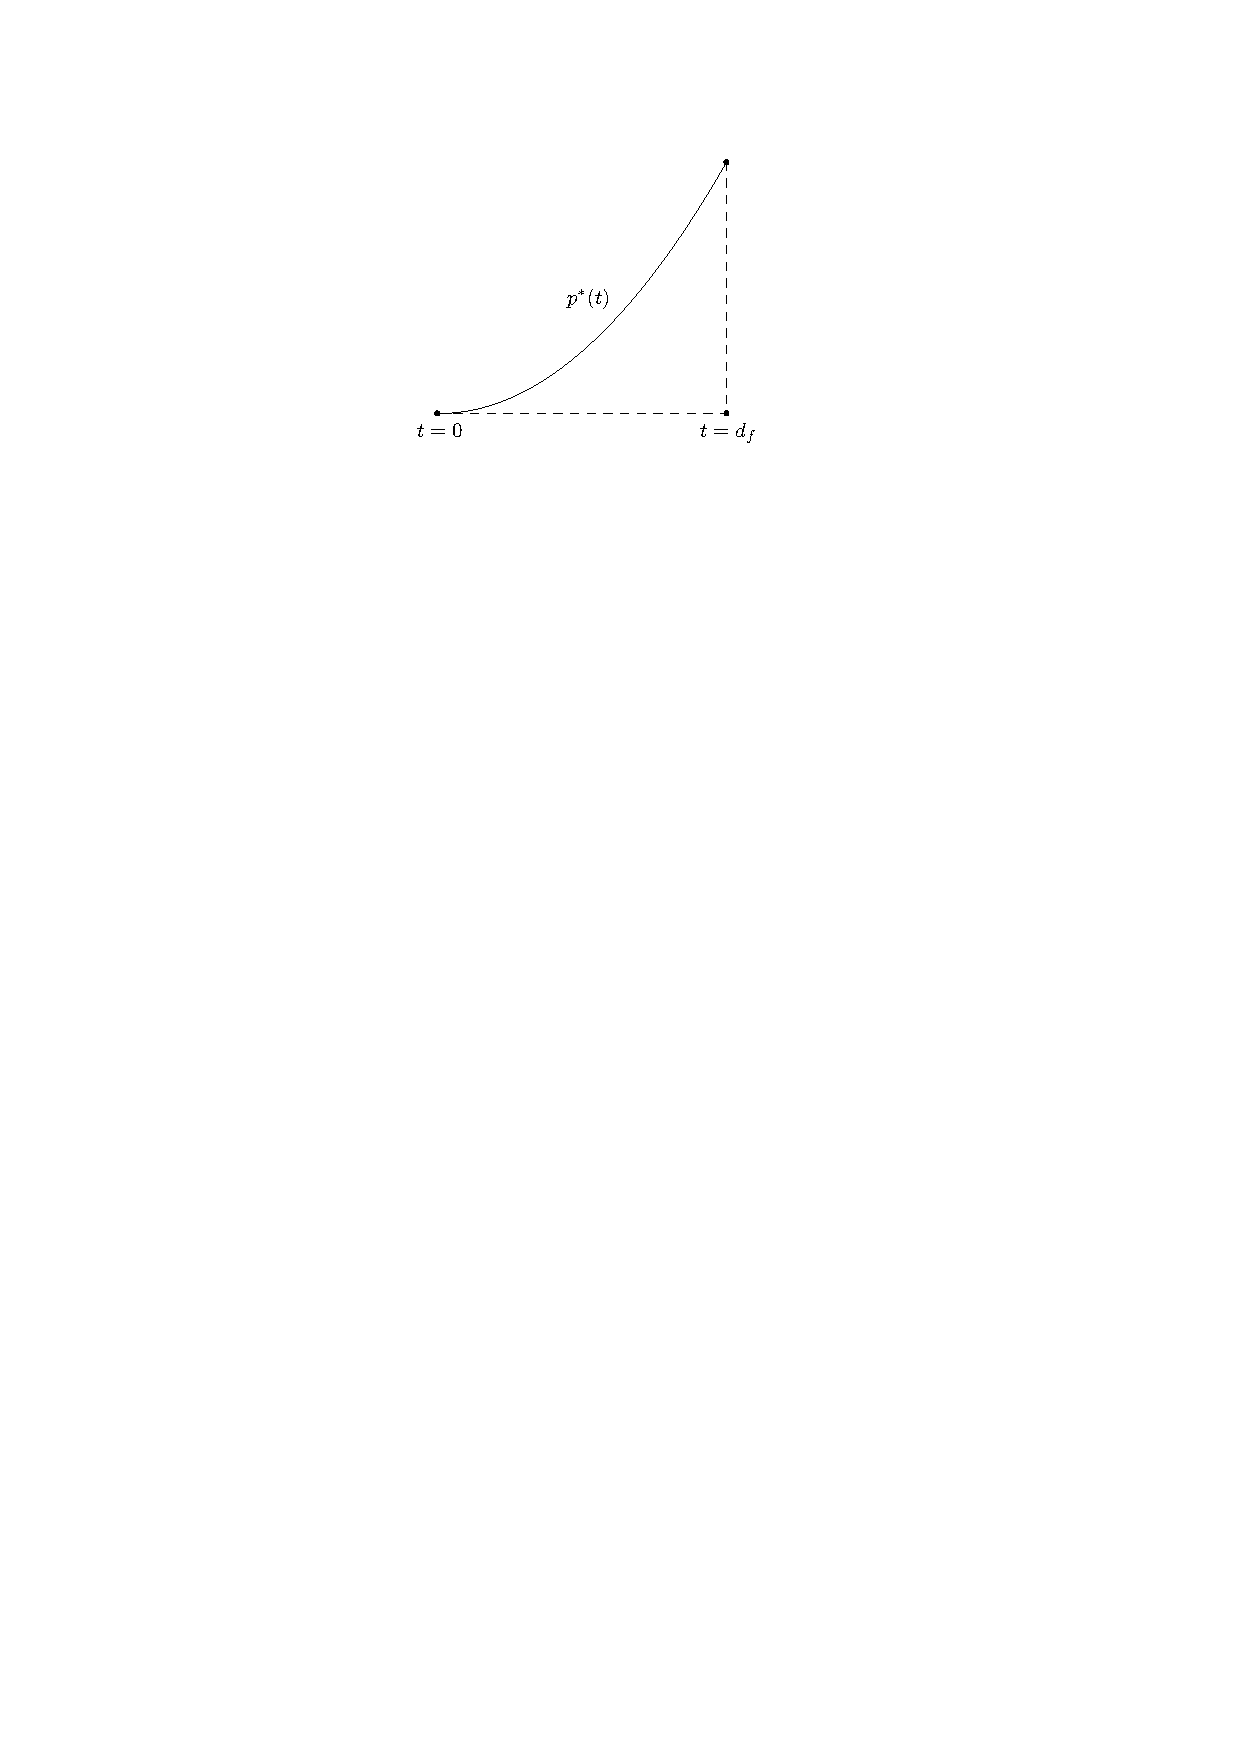
\includegraphics[scale=1]{figures/motion/acceleration}
  \caption{Full acceleration trajectory.}
  \label{fig:acceleration}
\end{figure}

We will start by assuming that the system contains a single vehicle, so that we
do not have to worry about keeping a safe distance to vehicle in front of it. We
will show how the bang-bang intervals, or \textit{bangs} for short, can be
obtained in this situation.
%
Without considering the boundary conditions, it follows from the vehicle
dynamics that the time it takes to fully accelerate from zero to maximum
velocity is given by
\begin{align*}
  T = v_{\max} / a_{\max} ,
\end{align*}
with corresponding trajectory $x^{*}$, given by
\begin{align*}
  x^{*}(t) = a_{\max} t^{2} / 2 \quad \text{ for }0 \leq t \leq T ,
\end{align*}
as illustrated in Figure~\ref{fig:acceleration}.
%
First, we introduce a some sort of state transformation that will prove to be
helpful. For position $x$ at time $t$, we define the corresponding \textit{schedule time}
by
\begin{align*}
  \bar{t}(t, x) := t - x / v_{\max} .
\end{align*}
In the following, we will use a bar above a symbol when dealing with schedule
time.
%
For example, time duration $T$ translated to schedule time, is given by
\begin{align*}
  \bar{T} &= \bar{t}(T, x^{*}(T)) - \bar{t}(0, 0) = T / 2 .
\end{align*}
{\color{blue} Transformation $\bar{t}$ induces equivalence classes in time-space, corresponding to lines with slope $v_{\max}$.}

The crossing of $v$ and $w$ in schedule time are given by $b = \bar{t}(0, 0)$
and $e = \bar{t}(t_{f}, x_{f})$, respectively.
%
Whenever $t_{f}$ is sufficiently large, it is clear that we need a full
deceleration and a full acceleration. Therefore, in schedule time, this would
take $2 \bar{T}$ time.
%
However, for smaller $t_{f}$, time of deceleration and acceleration need to
decrease equally. Therefore, writing $(x)^{+}$ for $\max(x, 0)$, the remaining
amount of schedule time in which we have zero acceleration is given by
\begin{align*}
  \bar{t}_{n} = {(e - b - 2\bar{T})}^{+}
\end{align*}
and the length of each bang is
\begin{align*}
  \bar{t}_{b} = (e - b - \bar{t}_{n}) / 2 ,
\end{align*}
so that the bangs are given by
\begin{align*}
  \bar{D} = (b, b + \bar{t}_{b}) , \\
  \bar{A} = (e - \bar{t}_{b}, e) .
\end{align*}
The corresponding trajectory are shown in Figure~\ref{fig:single_trajectory}.

\begin{figure}[t]
  \centering
\begin{subfigure}{0.4\textwidth}
    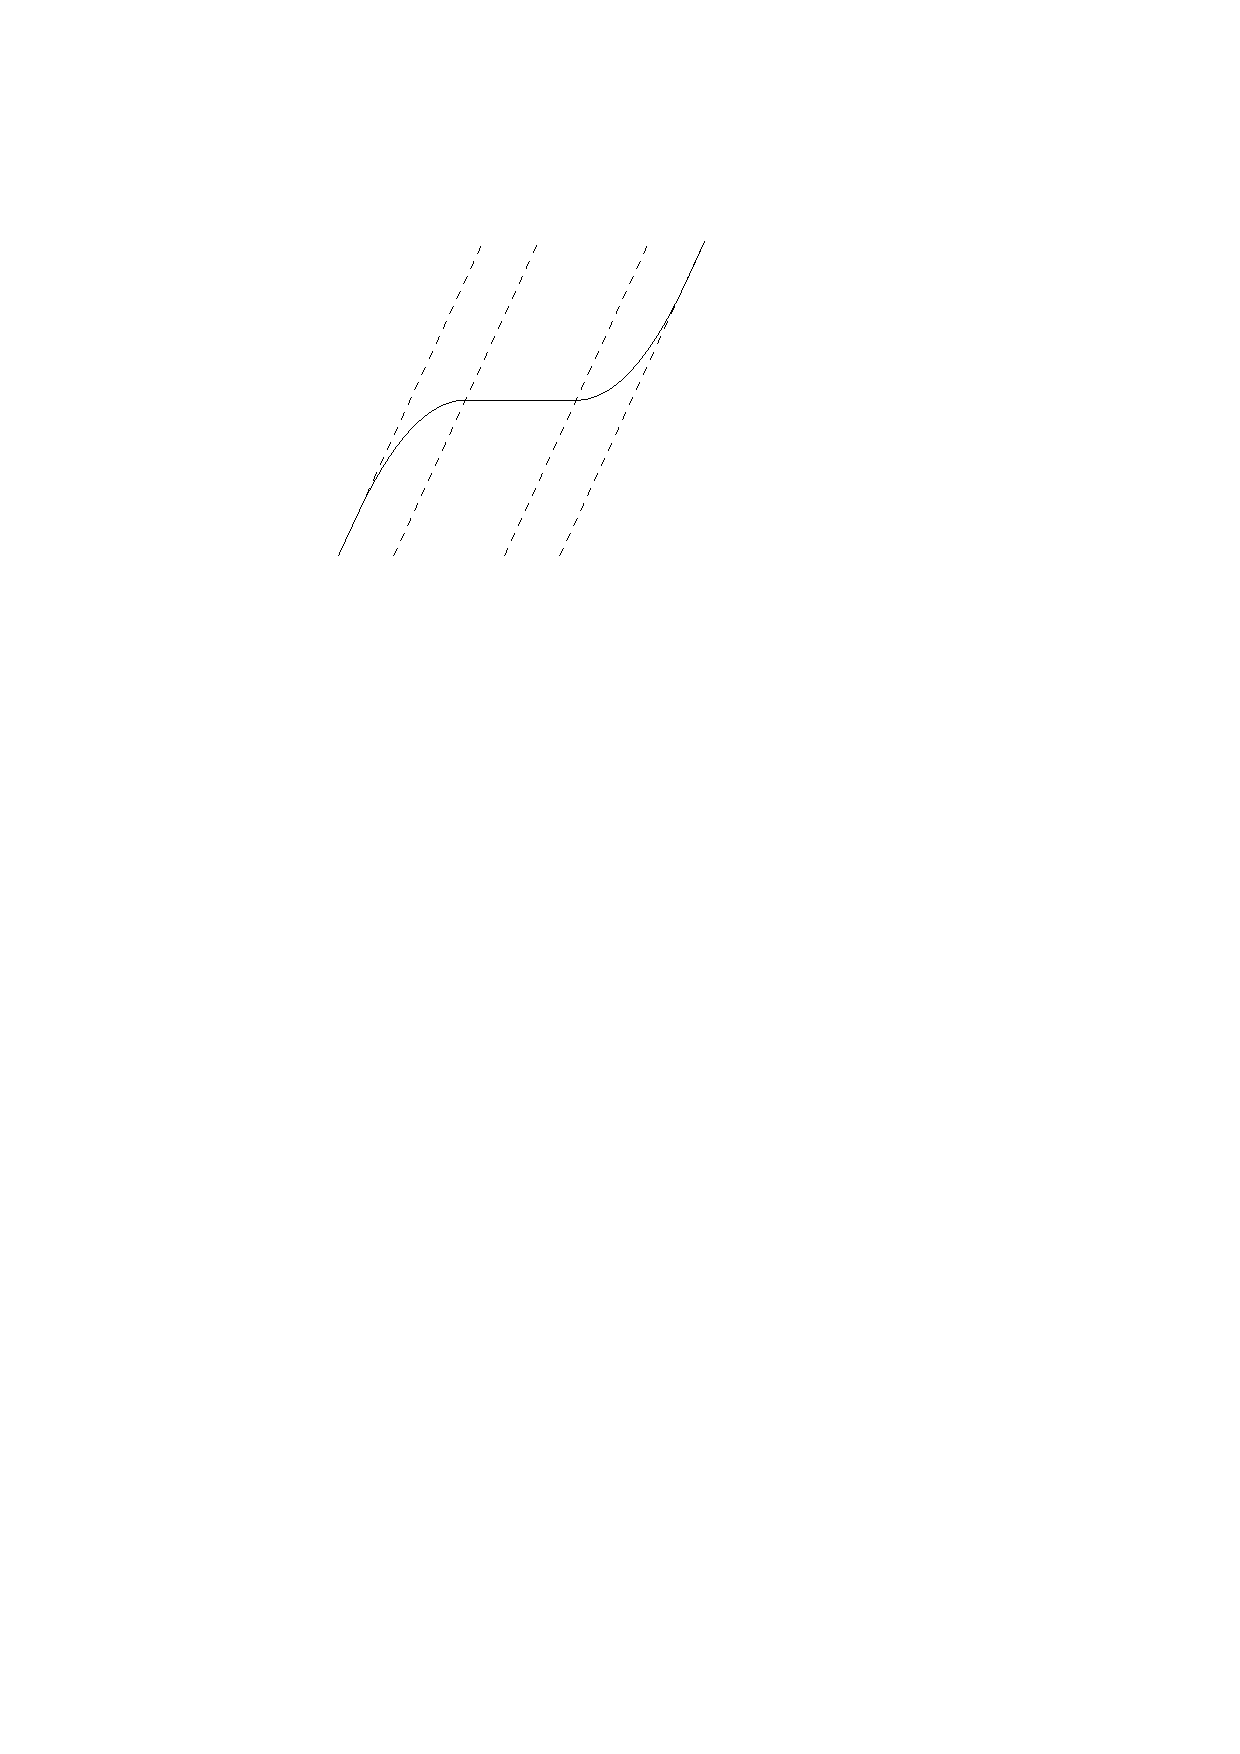
\includegraphics[scale=1]{figures/motion/single_trajectory_split}
    \caption{Positive waiting time $\bar{t}_{n} > 0$.}
    \label{fig:single_trajectory_split}
\end{subfigure}
\hfill
\begin{subfigure}{0.3\textwidth}
    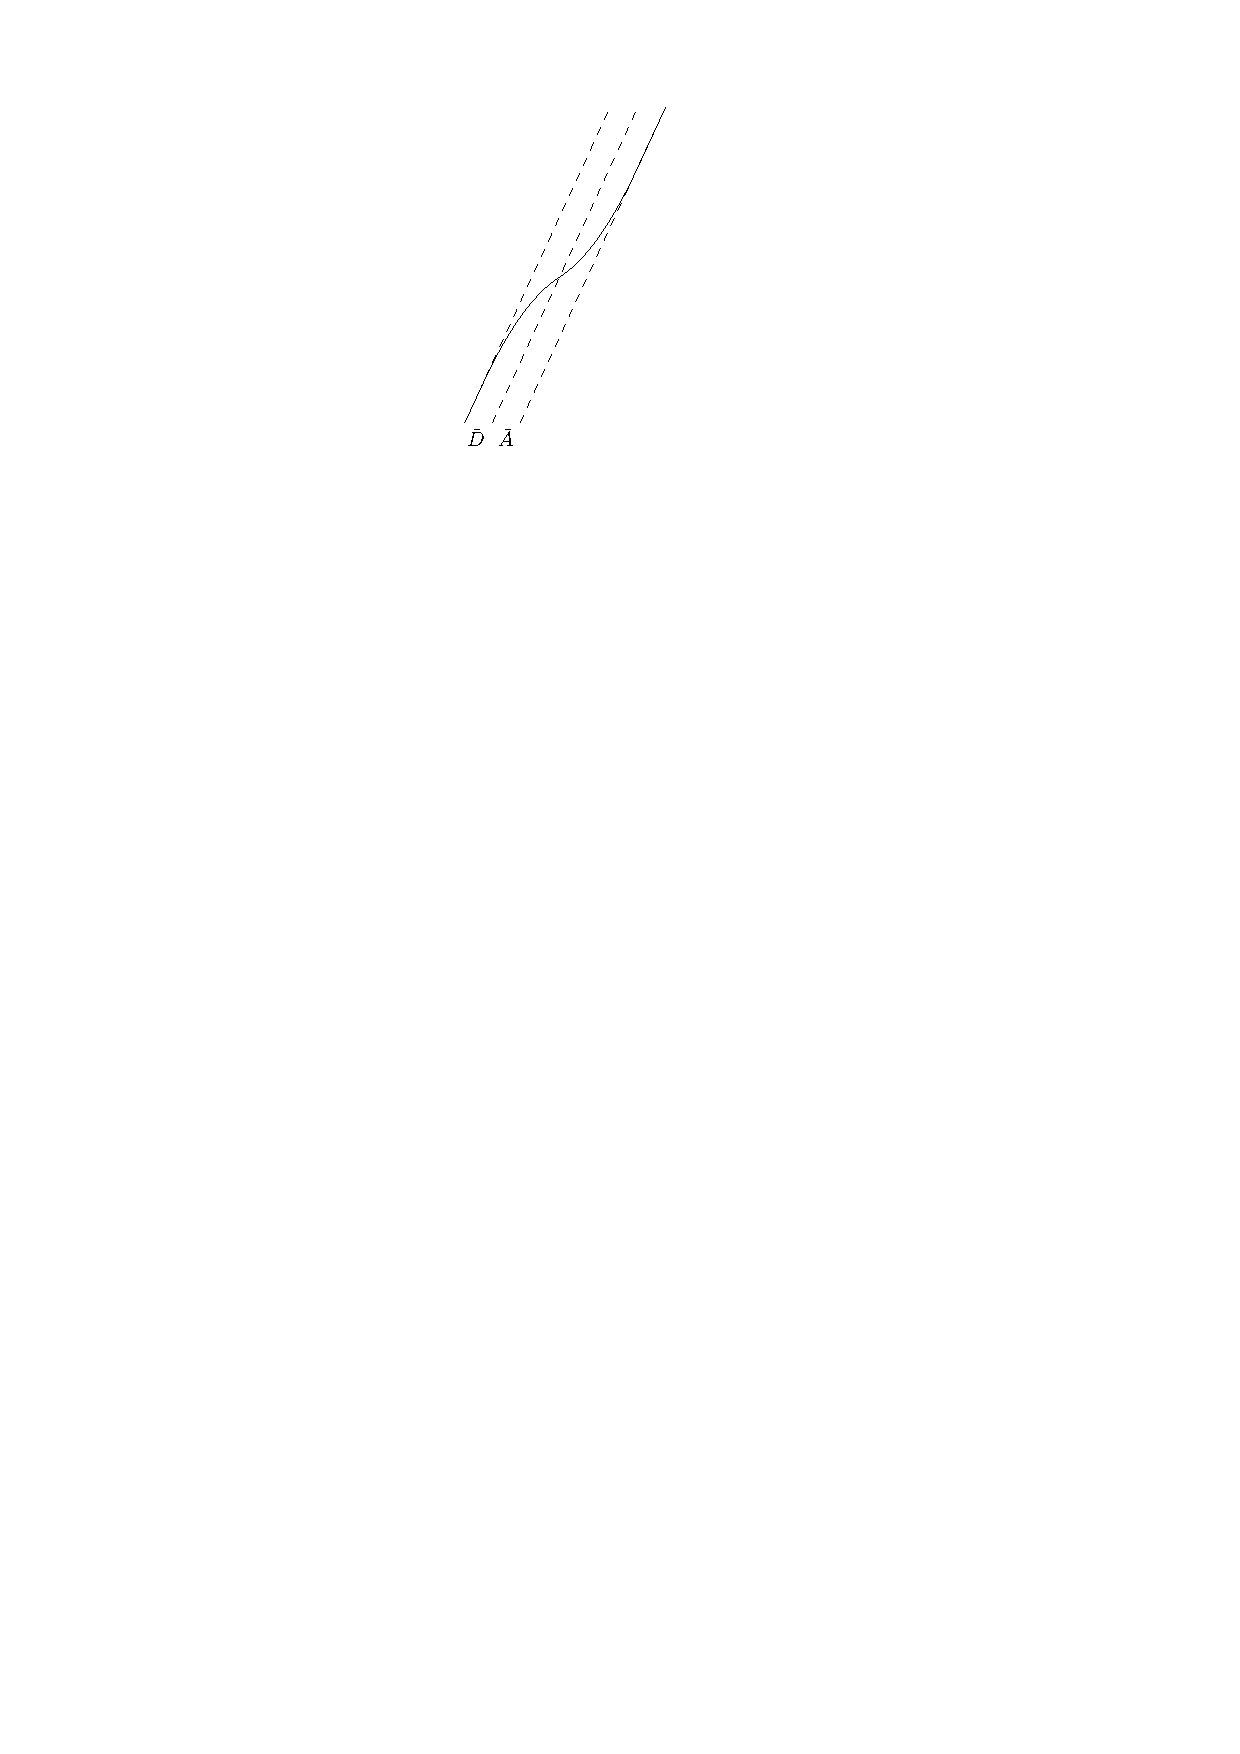
\includegraphics[scale=1]{figures/motion/single_trajectory_merged}
    \caption{Vehicle does not stop.}
    \label{fig:single_trajectory_merge}
\end{subfigure}
\caption{Optimal trajectory $x(t)$ for a single (isolated) vehicle with
  corresponding deceleration bang $\bar{D}$ and acceleration bang $\bar{A}$ in
  schedule time, in case the vehicle waits for some time (a) and in case the
  vehicle does not come to a full stop (b).}
  \label{fig:single_trajectory}
\end{figure}


\paragraph{Back to regular time.}
We are now left with translating these bangs back to the regular time scale. Let
the current velocity be denoted as $v_{c}$ and suppose $\bar{d}$ denotes the
duration of current acceleration bang in schedule time. Consider again the
full acceleration trajectory $x^{*}(t)$ on $0 \leq t \leq T$. Define
$t_{0}= v_{c} / a_{\max}$ so that we have $\dot{x}^{*}(t_{0}) = v_{c}$. Next, we
find $t_{1}$ such that $t_{0} \leq t_{1} \leq T$ and
\begin{align}
  \label{eq:regular}
   \bar{t}(t_{1}, x^{*}(t_{1})) - \bar{t}(t_{0}, x^{*}(t_{0})) = \bar{d} ,
\end{align}
such that the duration of the bang in regular time is given by $d = t_{1} - t_{0}$.
%
After some rewriting and substitution of the definitions of $x^{*}$ and
$\bar{t}$ in equation~\eqref{eq:regular}, we obtain the quadratic equation
\begin{align*}
  - \frac{a_{\max} t_{1}^{2}}{2 v_{\max}} + t_{1} - t_{0} + \frac{a_{\max} t_{0}^{2}}{2 v_{\max}} - \bar{d} = 0 ,
\end{align*}
for which we are interested in the solution
\begin{align*}
  t_{1} = T - \sqrt{T^{2} - 2T(t_{0} + \bar{d}) +t_{0}^{2}} .
\end{align*}

Similarly, for a deceleration bang of length $\bar{d}$ with current velocity
$v_{c}$, the duration is given by $d = t_{1} - t_{0}$ where
$t_{0} = (v_{\max} - v_{c}) / a_{\max}$ and $t_{1}$ is the solution to
\begin{align*}
  \bar{t}(t_{1}, -x^{*}(-t_{1})) - \bar{t}(t_{0}, -x^{*}(-t_{0})) = \bar{d} ,
\end{align*}
given by
\begin{align*}
  t_{1} = - T + \sqrt{T^{2} +2T(t_{0} + \bar{d}) + t_{0}^{2}} .
\end{align*}

Using the above formulas, we can translate a sequence of bangs in schedule time
to regular time. However, we need to be careful whenever the velocity becomes
$v_{\max}$, because the regular time is not unique in this case. Therefore, we
specify a \textit{target position} $x_{t}$, which fixes the regular time in
these cases as follows. Let $D=(b,e)$ be some deceleration bang, then the start
of the first deceleration bang in regular time is given by
\begin{align*}
  b + (x_{t} - x^{*}(T)) / v_{max} .
\end{align*}
%
The rest of the sequence of bangs in schedule time can now be translated as
follows, assuming that the velocity will not reach $v_{\max}$ until the last
acceleration bang. {\color{blue} We need to argue or prove why this assumption
  holds. Intuitively, if the assumption does not hold, the whole trajectory
  could be ``shifted up'' in the graph, which would decrease the objective.} We
keep track of the current time $t_{c}$ and velocity $v_{c}$. Each time we
process a bang $\bar{A}$ or $\bar{D}$, we update $v_{c} \leftarrow v_{c} \pm a_{\max} d$
accordingly, and $t \leftarrow t + d$, where $d$ is the regular bang duration, computed
using the formulas from above. This way, we obtain the sequence of bangs in
regular time, which completely define the corresponding controller.


\section*{Multiple vehicles}

\begin{figure}
  \centering
  \makebox[\textwidth][c]{% wider than textwidth
    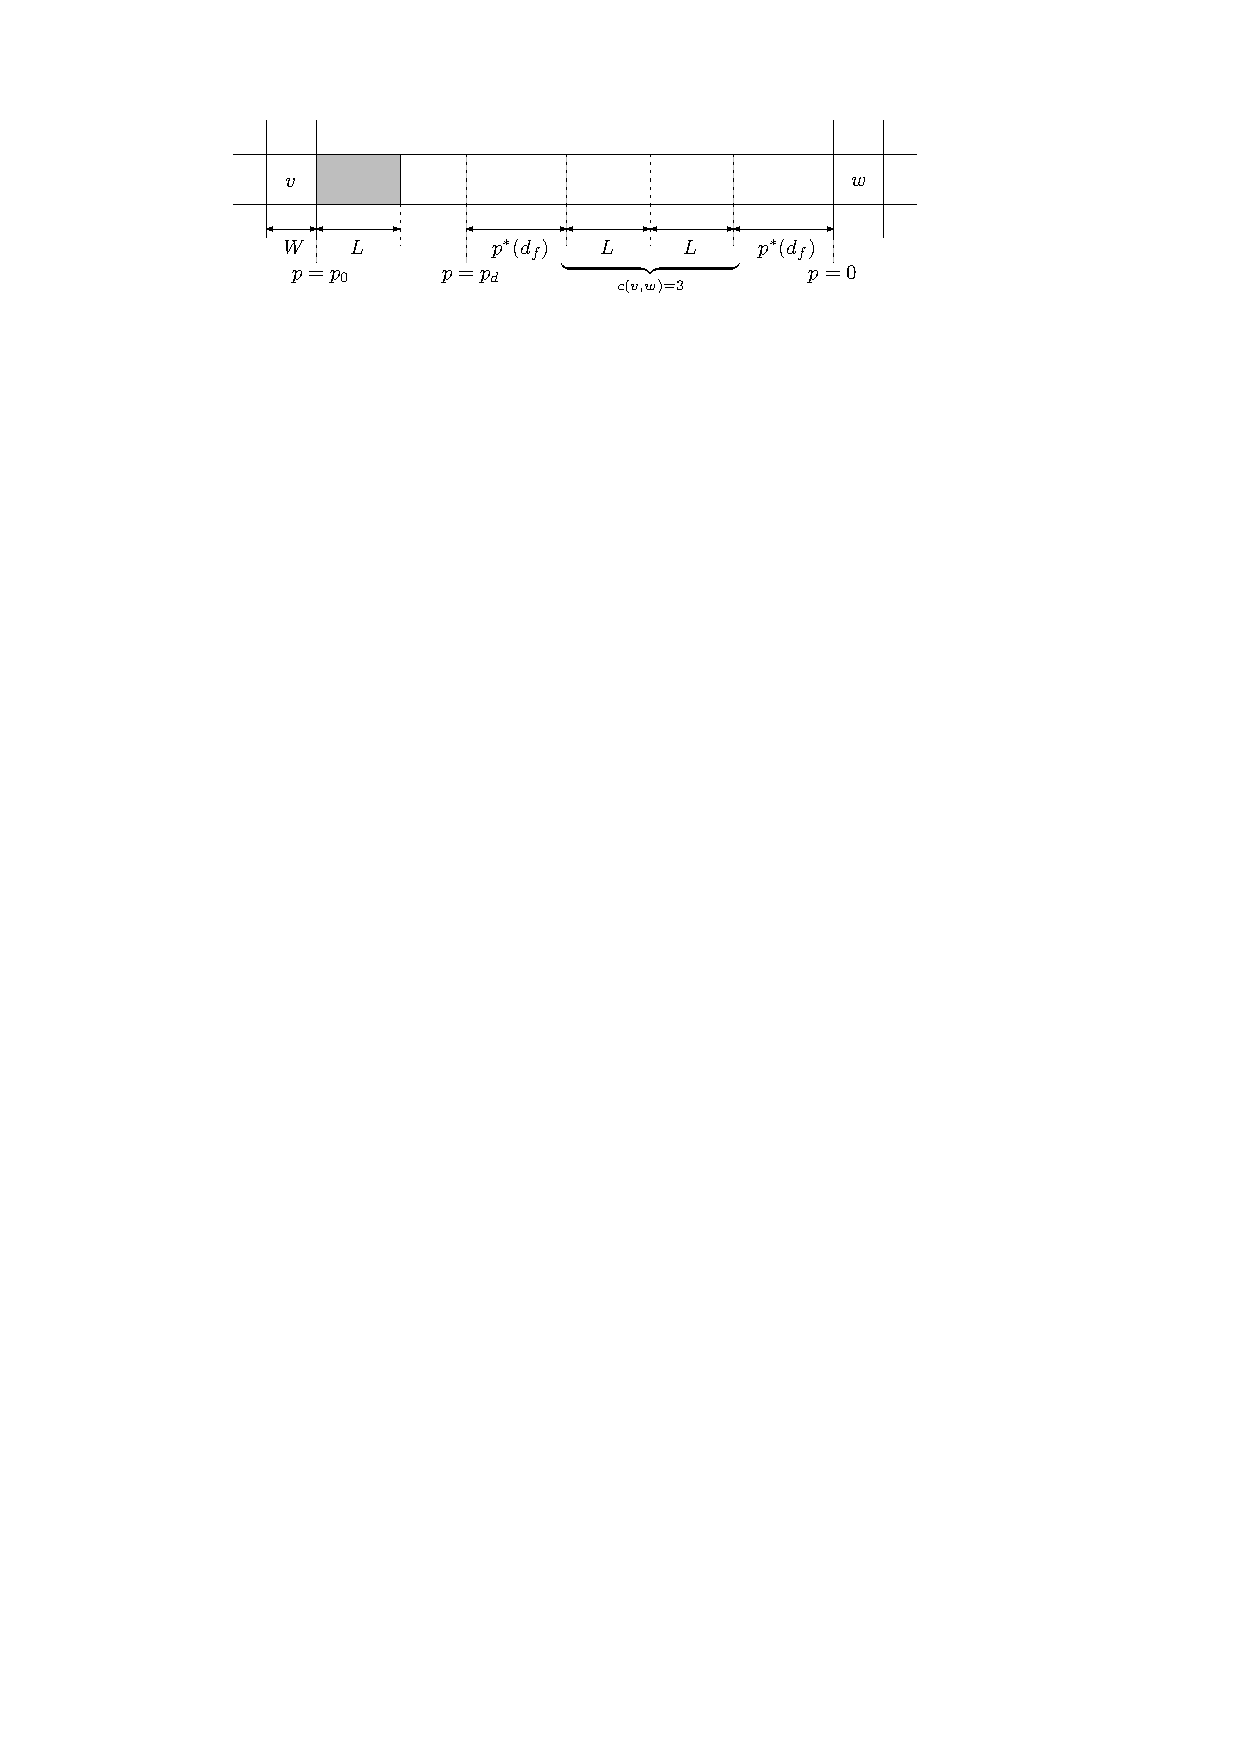
\includegraphics[width=1.1\textwidth]{figures/motion/tandem_annotated}
  }
  \caption{Tandem of intersections with indicated distances used in the capacity
    calculation.}
  \label{fig:tandem_annotated}
\end{figure}


We will now consider the case when the system contains multiple vehicles. Now,
we need to take into account the safe following constraints. This also causes
additional constraints to the crossing time scheduling problem, since the lane
only provides space for a limited number of vehicles, which we investigate
first.

\subsection*{Capacity}

Consider again the tandem of two intersection.
%
Suppose that we want to design the tandem network such that at least $c(v,w)$
vehicles can enter and decelerate to some waiting position, from which it is
also possible to accelerate again to full speed before crossing $w$.
%
Vehicles are required to drive at full speed $v=v_{\max}$ as long as they occupy
any intersection. Therefore, a vehicle crossing $v$ can only start decelerating
after $x(t) \geq L + W$, so the earliest position where a vehicle can come to a
stop is $x = L + W + x^{*}(T)$.
%
Because vehicles need to gain maximum speed $v=v_{\max}$ before reaching $w$,
the latest position where a vehicle can wait is $x_{f} - x^{*}(T)$.
%
Hence, in order to accomodate for $c(v,w)$ waiting vehicles, the length of the
lane must satisfy
\begin{align}
  d(v, w) \geq L + W + 2x^{*}(T) + (c(v,w) - 1) L ,
\end{align}
as illustrated in Figure~\ref{fig:tandem_annotated}.
%
Conversely, given the lane length $d(v,w)$, the corresponding capacity is given
by
\begin{align}
  c(v, w) = \texttt{floor}\left( \frac{d(v,w) - W - 2 x^{*}(T)}{L} \right) ,
\end{align}
where $\texttt{floor}(x)$ denotes the largest integer smaller than or equal to $x$.

\begin{remark}
  Without Assumption~\ref{assump1}, we cannot derive such a simple expression fo
  the capacity, because it would depend on the specific combination of lengths
  of the vehicles that arrived to the system.
\end{remark}


\subsection*{Bang merging}

Now assume we have a feasible crossing time schedule, that satisfies the buffer constraints.

We first describe the ``start-stop'' trajectory of a single vehicle, without
considering safe following constraints.
%
Observe that $L$ is the minimal distance between two consecutive vehicles. From
a waiting position, we move to the next waiting position that is exactly $L$
units further on the lane. It is clear that we need equal acceleration and
deceleration $\bar{D}=\bar{A}$. By symmetry, the vehicle moves $L/2$ during both
acceleration and deceleration.
%
Assume $L/2 < x^{*}(T)$, then we find $\bar{A}$.
{\color{blue} Still need to generalize this.}
Let $t_{0}$ be such that $x^{*}(t_{0}) = L/2$, then
\begin{align*}
t_{0} = \sqrt{L / a_{\max}} ,
\end{align*}
with corresponding schedule time
\begin{align*}
  \hat{t} = \bar{t}(t_{0}, L/2) = t_{0} - \frac{L}{2 v_{\max}} .
\end{align*}
Therefore, we have
\begin{align*}
  \bar{D} = (b, b + \hat{t}) , \\
  \bar{A} = (b + \hat{t}, b + 2 \hat{t}) .
\end{align*}

\begin{figure}
  \centering
  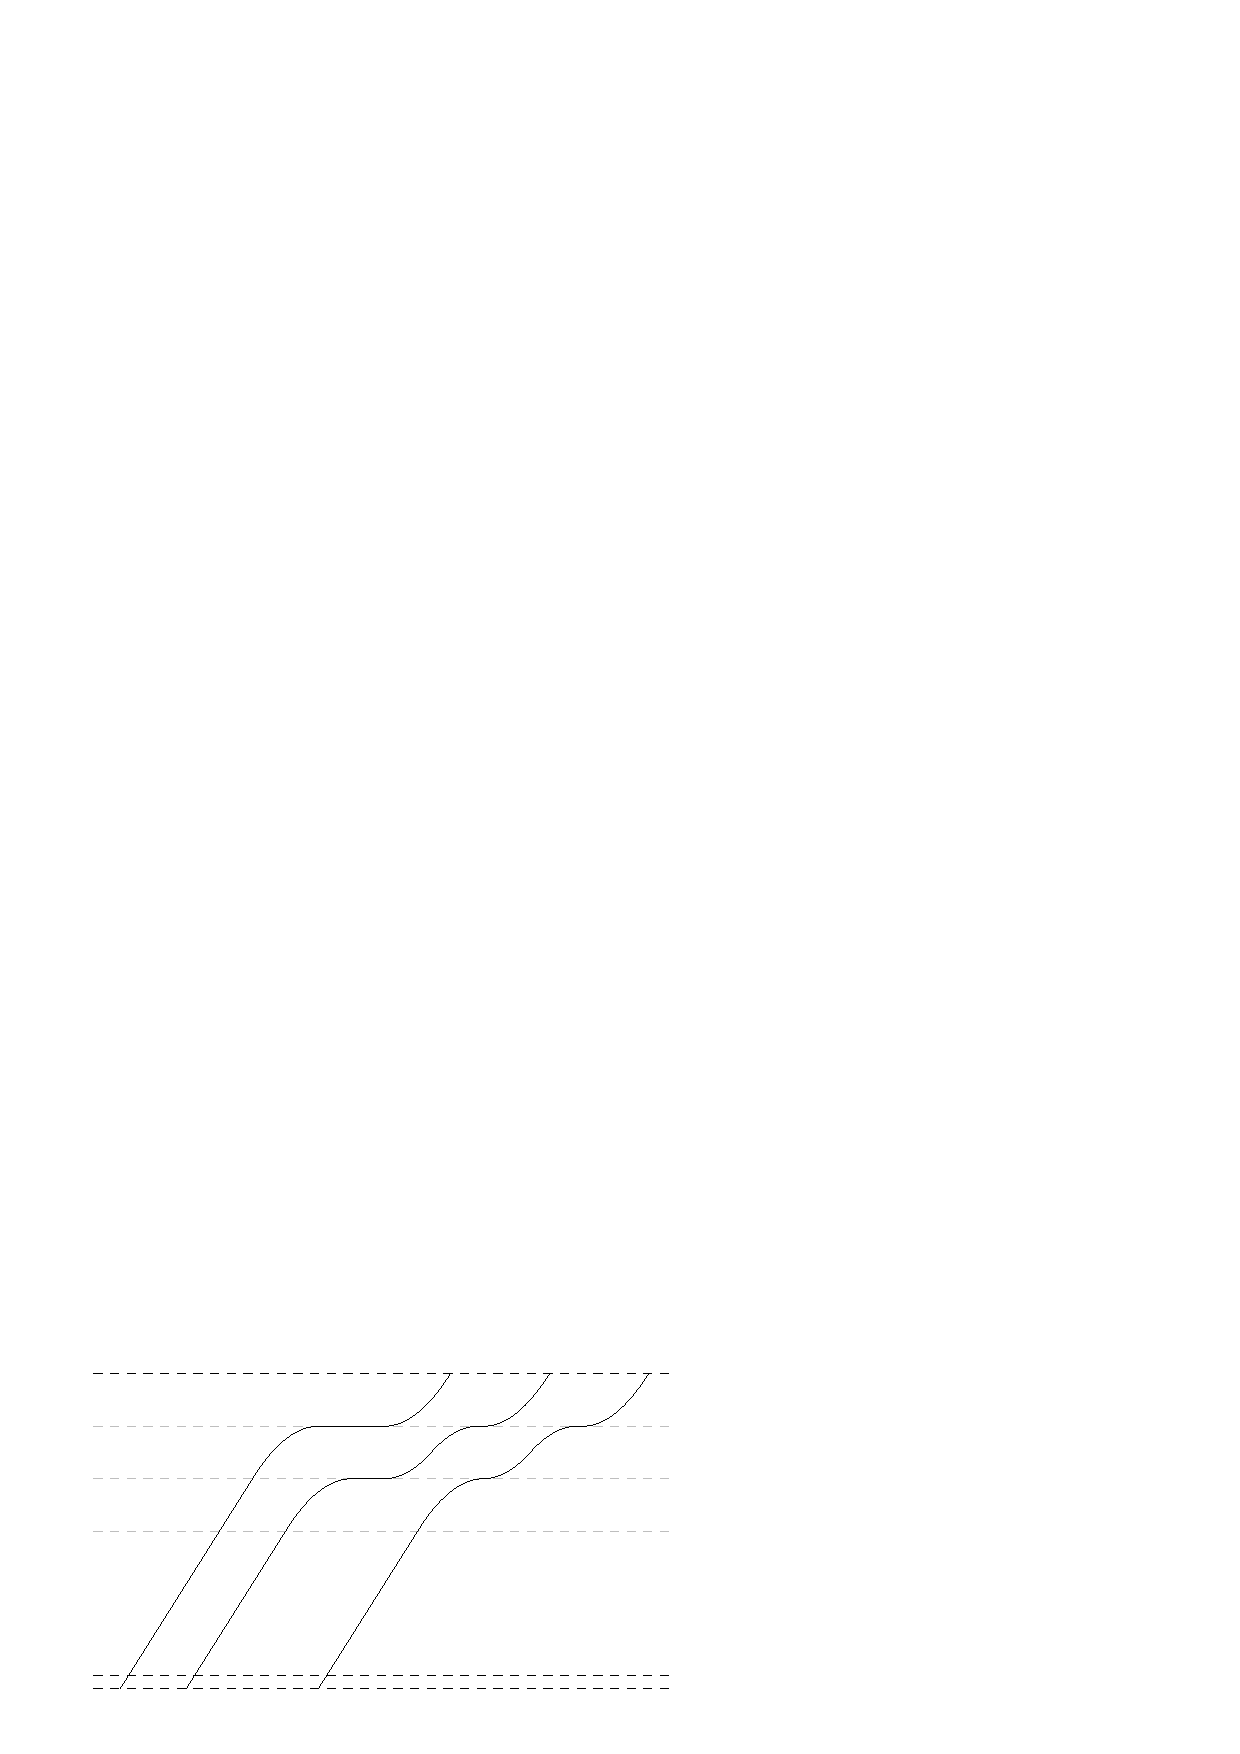
\includegraphics{figures/motion/buffer}
  \caption{Buffering vehicles.}
\end{figure}


\paragraph{Safe following constraints.}
We now see how the trajectory of the predecessor influences the bangs of the current vehicle.
Define
\begin{align*}
  \delta = L / v_{\max} .
\end{align*}


\end{document}
